% move all configuration stuff into one file so we can focus on the content
\documentclass[aspectratio=169,hyperref={pdfpagelabels=false,colorlinks=true,linkcolor=white,urlcolor=blue},t]{beamer}

%%%%%%%%%%%%%%%%%%%%%%%%%%%%%%%%%%%%%%%%%%%%%%%%%%%%%%%%%%%%%%%%%%%%%%%%%%%%%%%%%%
%%%%%%%%%%%%%%%%%%%%%%%%%%%%%%%%%%%%%%%%%%%%%%%%%%%%%%%%%%%%%%%%%%%%%%%%%%%%%%%%%%
% packages
\usepackage{pict2e}
\usepackage{epic}
\usepackage{amsmath,amsfonts,amssymb}
\usepackage{units}
\usepackage{fancybox}
\usepackage[absolute,overlay]{textpos} 
\usepackage{media9} % avi2flv: "C:\Program Files\ffmpeg\bin\ffmpeg.exe" -i TuneFreqFilterbank.avi -b 600k -s 441x324 -r 15 -acodec copy TuneFreqFilterbank.flv
\usepackage{animate}
\usepackage{gensymb}
\usepackage{multirow}
\usepackage{silence}
\usepackage[backend=bibtex,style=ieee]{biblatex}
\AtEveryCitekey{\iffootnote{\tiny}{}}
\addbibresource{references}

%%%%%%%%%%%%%%%%%%%%%%%%%%%%%%%%%%%%%%%%%%%%%%%%%%%%%%%%%%%%%%%%%%%%%%%%%%%%%%%%%%
%%%%%%%%%%%%%%%%%%%%%%%%%%%%%%%%%%%%%%%%%%%%%%%%%%%%%%%%%%%%%%%%%%%%%%%%%%%%%%%%%%
% relative paths
\graphicspath{{graph/}}


%%%%%%%%%%%%%%%%%%%%%%%%%%%%%%%%%%%%%%%%%%%%%%%%%%%%%%%%%%%%%%%%%%%%%%%%%%%%%%%%%%
%%%%%%%%%%%%%%%%%%%%%%%%%%%%%%%%%%%%%%%%%%%%%%%%%%%%%%%%%%%%%%%%%%%%%%%%%%%%%%%%%%
% units
\setlength{\unitlength}{1mm}

%%%%%%%%%%%%%%%%%%%%%%%%%%%%%%%%%%%%%%%%%%%%%%%%%%%%%%%%%%%%%%%%%%%%%%%%%%%%%%%%%%
%%%%%%%%%%%%%%%%%%%%%%%%%%%%%%%%%%%%%%%%%%%%%%%%%%%%%%%%%%%%%%%%%%%%%%%%%%%%%%%%%%
% theme & layout
\usetheme{Frankfurt}
\beamertemplatenavigationsymbolsempty
%\setbeamertemplate{frametitle}[smoothbars theme]
\setbeamertemplate{frametitle}
{
    \begin{beamercolorbox}[ht=1.8em,wd=\paperwidth]{frametitle}
        \vspace{-.1em}%
        \hspace{.2em}{\strut\insertframetitle\strut}
        
        \hspace{.2em}\small\strut\insertframesubtitle\strut
        %\hfill
        %
\includegraphics[height=.8cm,keepaspectratio]{CenterMusicTechnology-solid-2lines-white-CoAtag}
        
    \end{beamercolorbox}
    \begin{textblock*}{100mm}(11.6cm,.7cm)
        \includegraphics[height=.8cm,keepaspectratio]{logo_GTCMT_black}
    \end{textblock*}
}

% set this to ensure bulletpoints without subsections
\usepackage{remreset}
\makeatletter
\@removefromreset{subsection}{section}
\makeatother
\setcounter{subsection}{1}

%---------------------------------------------------------------------------------
% appearance
\setbeamercolor{structure}{fg=gtgold}
\setbeamercovered{transparent} %invisible
\setbeamercolor{bibliography entry author}{fg=black}
\setbeamercolor*{bibliography entry title}{fg=black}
\setbeamercolor*{bibliography entry note}{fg=black}

%\usepackage{pgfpages}
%\setbeameroption{show notes}
%\setbeameroption{show notes on second screen=right}
%---------------------------------------------------------------------------------
% fontsize
\let\Tiny=\tiny

%%%%%%%%%%%%%%%%%%%%%%%%%%%%%%%%%%%%%%%%%%%%%%%%%%%%%%%%%%%%%%%%%%%%%%%%%%%%%%%%%%
%%%%%%%%%%%%%%%%%%%%%%%%%%%%%%%%%%%%%%%%%%%%%%%%%%%%%%%%%%%%%%%%%%%%%%%%%%%%%%%%%%
% warnings
\pdfsuppresswarningpagegroup=1
\WarningFilter{biblatex}{Patching footnotes failed}
\WarningFilter{latexfont}{Font shape}
\WarningFilter{latexfont}{Some font shapes}
\WarningFilter{gensymb}{Not defining}



\subtitle{Part 9.2: Music Similarity and Mood Recognition}

%%%%%%%%%%%%%%%%%%%%%%%%%%%%%%%%%%%%%%%%%%%%%%%%%%%%%%%%%%%%%%%%%%%%%%%%%%%%
\begin{document}
    % generate title page
	

\begin{frame}
    \titlepage
    %\vspace{-5mm}
    \begin{flushright}
        \href{http://www.gtcmt.gatech.edu}{\includegraphics[height=.8cm,keepaspectratio]{logo_GTCMT_black}}
    \end{flushright}
\end{frame}


    \section[overview]{lecture overview}
        \begin{frame}{temporal analysis}{overview}
            \begin{itemize}
                \item   \textbf{text book}  
                    \begin{itemize}
                        \item   \href{http://ieeexplore.ieee.org/xpl/articleDetails.jsp?tp=&arnumber=6331125&}{\underline{\textit{Chapter 8: Musical Genre, Similarity, and Mood} (pp.~156--162)}}
                    \end{itemize}
                \item   \textbf{sources}: slides (latex) \& Matlab  
                    \begin{itemize}
                        \item   \href{https://github.com/alexanderlerch/ACA-Slides}{\underline{github repository}}
                    \end{itemize}
                \bigskip
                \item<2->   \textbf{lecture content}
                    \begin{itemize}
                        \item<2->  music similarity 
                        \item<3->  k-means clustering and SOMs 
                        \item<4->  mood and emotion
                        \item<5->  linear regression
                    \end{itemize}
            \end{itemize}
        \end{frame}

    \section[intro]{introduction}
        \begin{frame}{similarity and mood}{introduction}
            \begin{itemize}
                \item	\textbf{commonalities} with genre classification
                    \begin{itemize}
                        \item	similar set of features
                        \item	ambiguous 'ground truth'
                        \item   unclear value/impact of low level and high level features
                    \end{itemize}
                \bigskip
                \item<2->	 \textbf{differences} to genre classification
                    \begin{itemize}
                        \item	\textit{mood}: often not a classification but regression
                        \item	\textit{similarity}: distance measure instead of categorizing into classes
                    \end{itemize}
            \end{itemize}
        \end{frame}


    \section[similarity]{audio similarity}
        \begin{frame}{audio similarity}{introduction}
            \begin{itemize}
                \item   \textbf{perception} of music similarity
                    \begin{itemize}
                        \item	multi-dimensional (melodic, rhythmic, sound quality, \ldots)
                        \item	user dependent
                        \item	associative, may also depend on editorial data
                        \item	may be context dependent
                    \end{itemize}
                \bigskip
                \item<2->   genres are \textbf{clusters of musical similarity}
                \item[$\Rightarrow$]	genre classification is a \textit{special case} of audio similarity measures
                \item<3->	instead of assigning (genre) labels, the similarity/distance between (pairs) of files is measured
            \end{itemize}
        \end{frame}

        \begin{frame}{audio similarity}{K-Means clustering example}
            \begin{itemize}
                \item   simple k-means example
                    \begin{itemize}
                        \item   \textbf{goal}: minimize intra-cluster variance
                        \item   \textbf{distance}: Euclidean
                        \item   \textbf{procedure}:
                            \begin{enumerate}
                                \item	\textit{initialization}:\\ randomly select $K$ points in the feature space as initialization.
                                \item<2->	\textit{assignment}:\\ assign each observation to the cluster with the mean/centroid of the closest cluster.
                                \item<3->	\textit{update}:\\ compute mean/centroid for each cluster.
                                \item<4->	\textit{iteration}:\\ go to step $2$ until the clusters converge.
                            \end{enumerate}
                    \end{itemize}
            \end{itemize}
        \end{frame}
        \begin{frame}{audio similarity}{K-Means clustering example}
            \setcounter{i}{0}
            \setcounter{j}{1}
            \whiledo{\value{i}<6}
            {
                \only<\value{j}>{\figwithref{KMeans-\arabic{i}}{matlab source: matlab/displayKMeans.m}}
                \stepcounter{i}
                \stepcounter{j}
            }
            \only<1>{
                \begin{itemize}
                    \item   data points
                \end{itemize}
                }
            \only<2>{
                \begin{itemize}
                    \item   init
                    \item   assignment
                \end{itemize}
                }
            \only<3-5>{
                \begin{itemize}
                    \item   update centroids
                    \item   assignment
                \end{itemize}
                }
            \only<6>{
                \begin{itemize}
                    \item   convergence
                \end{itemize}
                }
        \end{frame}
        \begin{frame}{audio similarity}{visualization in a 2D space}
            \begin{itemize}
                \item \textbf{problem}
                    \begin{itemize}
                        \item   feature space is high-dimensional
                        \item[$\rightarrow$] cannot be visualized
                    \end{itemize}
                \bigskip
                \item<2-> find \textbf{mapping} to 2D ``preserving'' (high-dimensional) distance metrics
            \end{itemize}
        \end{frame}
            
        \begin{frame}{audio similarity}{visualization example: SOM 1/2}
                    \begin{enumerate}
                        \item	create a map with 'neurons'
                        \item<2->	train
                                \begin{itemize}
                                    \item	for each training sample find BMU (best matching unit)
                                    \item	adapt BMU and neighbors toward training sample
                                    \begin{equation*}
                                        W_v(t + 1) = W_v(t) + \theta (v, t) \alpha(t)\big(D(t) - W_v(t)\big)
                                    \end{equation*}
                                    \begin{footnotesize}
                                        \begin{itemize}
                                            \item	$\theta (v, t)$: depends on distance from BMU
                                            \item	$\alpha (t)$: learning restraint
                                            \item	$D(t)$ training sample
                                        \end{itemize}
                                    \end{footnotesize}
                                \end{itemize}
                    \end{enumerate}
                    \only<2->{
                    \begin{figure}
                        \centering
                            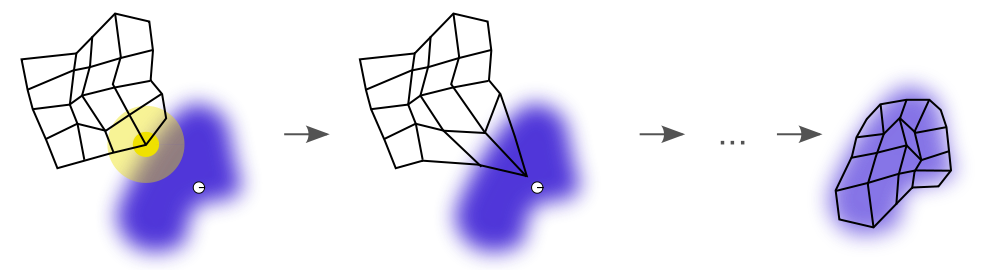
\includegraphics[scale=.3]{graph/SOM_training}
                    \end{figure}
                    \addreference{\url{https://en.wikipedia.org/wiki/Self-organizing_map}}}
        \end{frame}
        \begin{frame}{audio similarity}{SOM 2/2}
                    \begin{figure}
                        \centering
                            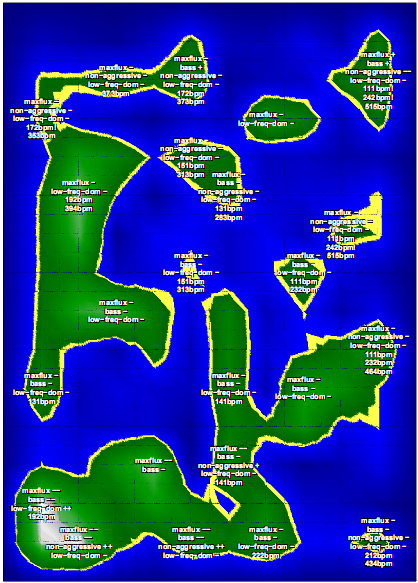
\includegraphics[scale=.3]{graph/som}
                    \end{figure}
                    from \footfullcite{pampalk_islands_2001}
        \end{frame}


    \section[mood]{mood recognition}

        \begin{frame}{mood recognition}{introduction}
            
            \begin{itemize}
                \item	\textbf{objective}:identify mood/emotion of a song
                \item<2->   \textbf{terminology}:
                    \begin{itemize}
                        \item \textit{Music Mood Recognition} and \textit{Music Emotion Recognition} usually used simultaneously
                    \end{itemize}
            \end{itemize}
            
            \question{What is the difference between \textit{mood} and \textit{emotion}}
            \begin{itemize}
                \item	\textit{emotion}: 
                    \begin{itemize}
                        \item   temporary, evanescent
                        \item   (directly) related to external stimuli
                    \end{itemize}
                \item	\textit{mood}: 
                    \begin{itemize}
                        \item   longer term, stable
                        \item   diffuse affect state
                    \end{itemize}
            \end{itemize}
        \end{frame}
            
        \begin{frame}{mood recognition}{challenges}
            \begin{itemize}
                \item   \textbf{ground truth data}
                    \begin{itemize}
                        \item   \textit{verbalization} of emotions/moods usually misleading
                        \item   not easily \textit{quantifiable}/categorizable
                        \item   change over time?
                    \end{itemize}
                \bigskip
                \item   \textbf{research focus}
                    \begin{itemize}
                        \item<2->	can established \textit{basic emotions} (happiness, anger, fear, \ldots) used for music perception
                        \item<3->	\textit{aroused vs.\ transported} moods?
                    \end{itemize}
            \end{itemize}
        \end{frame}
                
        \begin{frame}{mood recognition}{models}
            \begin{itemize}
                \item	classification into \textbf{label clusters}
                
                    \only<1>{
                    \begin{scriptsize}
                    \begin{tabular}{ccccc}
                        \\ \hline
                        \bf{\emph{Cluster 1}}	 & \bf{\emph{Cluster 2}}	 & \bf{\emph{Cluster 3}}	 & \bf{\emph{Cluster 4}}	 & \bf{\emph{Cluster 5}}\\ 
                         \hline
                        \bf{\textnormal{Rowdy}}	 & Amiable/Good Natured	 & Literate	 & Witty	 & Volatile\\
                        \bf{\textnormal{Rousing}}	 & Sweet	 & Wistful	 & Humorous	 & Fiery\\
                        \bf{\textnormal{Confident}}	 & Fun	 & Bittersweet	 & Whimsical	 & Visceral\\
                        \bf{\textnormal{Boisterous}}	 & Rollicking	 & Autumnal	 & Wry	 & Aggressive\\
                        \bf{\textnormal{Passionate}}	 & Cheerful	 & Brooding	 & Campy	 & Tense/Anxious\\
                        \bf{}	 & 	 & Poignant	 & Quirky	 & Intense\\
                        \bf{}	 & 	 & 	 & Silly	 & \\
                    \end{tabular}
                    \end{scriptsize}
                    }
                \item<2->	\textbf{mood model}, circumplex model most common\footfullcite{russel_circumplex_1980}
                    \only<2>{
                    \begin{figure}
                        \centering
                            \includegraphics[scale=.3]{graph/circumplex_affect}
                    \end{figure}
                    }
            \end{itemize}
        \end{frame}
                
        \begin{frame}{mood recognition}{mood model: regression modeling}
            \begin{itemize}
                \item   \textbf{mapping} 
                    \begin{itemize}
                        \item (N-dimensional) observation (feature) to 2-dimensional coordinate (valence/arousal)
                    \end{itemize}
                \bigskip
                \item   \textbf{training}
                    \begin{itemize}
                        \item find model to minimize error between data points and ``prediction''
                    \end{itemize}
            \end{itemize}
        \end{frame}
                
        \begin{frame}{linear regression}{introduction to regression 1/2}
                    \begin{itemize}
                        \item fit a linear function to a series of points  $(x_j,y_j)$
                            \begin{equation*}
                                y_n = m\cdot x_n + b
                            \end{equation*}
                    \end{itemize}
                \figwithref{LinearRegression}{\url{https://en.wikipedia.org/wiki/Linear_regression}}
        \end{frame}
                
        \begin{frame}{linear regression}{introduction to regression 2/2}
            \begin{itemize}
                \item   minimize error between model and data (here: least squares)
            \end{itemize}
            \begin{scriptsize}
            \begin{eqnarray*}
                e_n^2 &=& (y_n - mx_n - b)^2\\
                E &=& \sum (y_n - mx_n - b)^2\\
            \end{eqnarray*}
            \vspace{-10mm}
            \begin{columns}[T]
                \column{.5\linewidth}
                    \begin{eqnarray*}
                        \visible<2->{\frac{\partial E}{\partial b} = \sum -2(y_n - mx_n - b) &=& 0}\\
                        \visible<3->{-2\sum y_n +2\sum mx_n +2\sum b &=& 0}\\
                        \visible<4->{\sum mx_n + \sum b &=& \sum y_n}\\
                        \visible<5->{m\sum x_n + \mathcal{N}b &=& \sum y_n}
                    \end{eqnarray*}
                \column{.5\linewidth}
                    \begin{eqnarray*}
                        \visible<2->{\frac{\partial E}{\partial m} = \sum -2x_n(y_n - mx_n - b) =& 0&}\\
                        \visible<3->{-2\sum x_ny_n +2\sum mx_n^2 +2\sum bx_n =& 0&}\\
                        \visible<4->{\sum mx_n^2 + \sum bx_n = \sum x_ny_n&&}\\
                        \visible<5->{m\sum x_n^2 + b\sum x_n = \sum x_ny_n&&}
                    \end{eqnarray*}
            \end{columns}
            \bigskip
            \bigskip
            \visible<6>{
            \begin{eqnarray*}
                &\Rightarrow&\\
                m &=& \frac{\mathcal{N}\sum x_ny_n-\sum x_n\sum y_n}{\mathcal{N}\sum x_n^2 -\left(\sum x_n\right)^2}\\
                b &=& \frac{\sum y_n}{\mathcal{N}}-m\frac{\sum x_n}{\mathcal{N}}\\
            \end{eqnarray*}
            }
            \end{scriptsize}
        \end{frame}

        \begin{frame}{mood recognition}{range of results}
            \begin{itemize}
                \item	\textbf{5 mood clusters}:\\ 40--60\% classification rate
                \bigskip
                \item	\textbf{mood model}:\\ 0.1--0.4 absolute prediction error (unit circle)
            \end{itemize}
        \end{frame}


    \section[summary]{lecture summary}
        \begin{frame}{summary}{lecture content}
            \begin{enumerate}
                \item   what are typical use cases for music similarity and mood recognition
                \smallskip
                \item<2->   discuss advantages and disadvantages of using classes vs the circumplex model for mood recognition
            \end{enumerate}
        \end{frame}
\end{document}

